\documentclass[11pt]{article}

\usepackage{epsilonj}

\RequirePackage{graphicx}
\RequirePackage{wrapfig}
\RequirePackage[colorlinks,citecolor=blue,urlcolor=blue]{hyperref}

\date{\vspace{-5ex}}

\begin{document}
	
	\TITLE{Весёлый уголок}
	\SHORTTITLE{Весёлый уголок}
	
	\AUTHOR{}{}
	\SHORTAUTHOR{}
	
\DoFirstPageTechnicalStuff

\section{Дорожный знак}

\begin{wrapfigure}{r}{5cm}\centering\vspace{-2ex}
	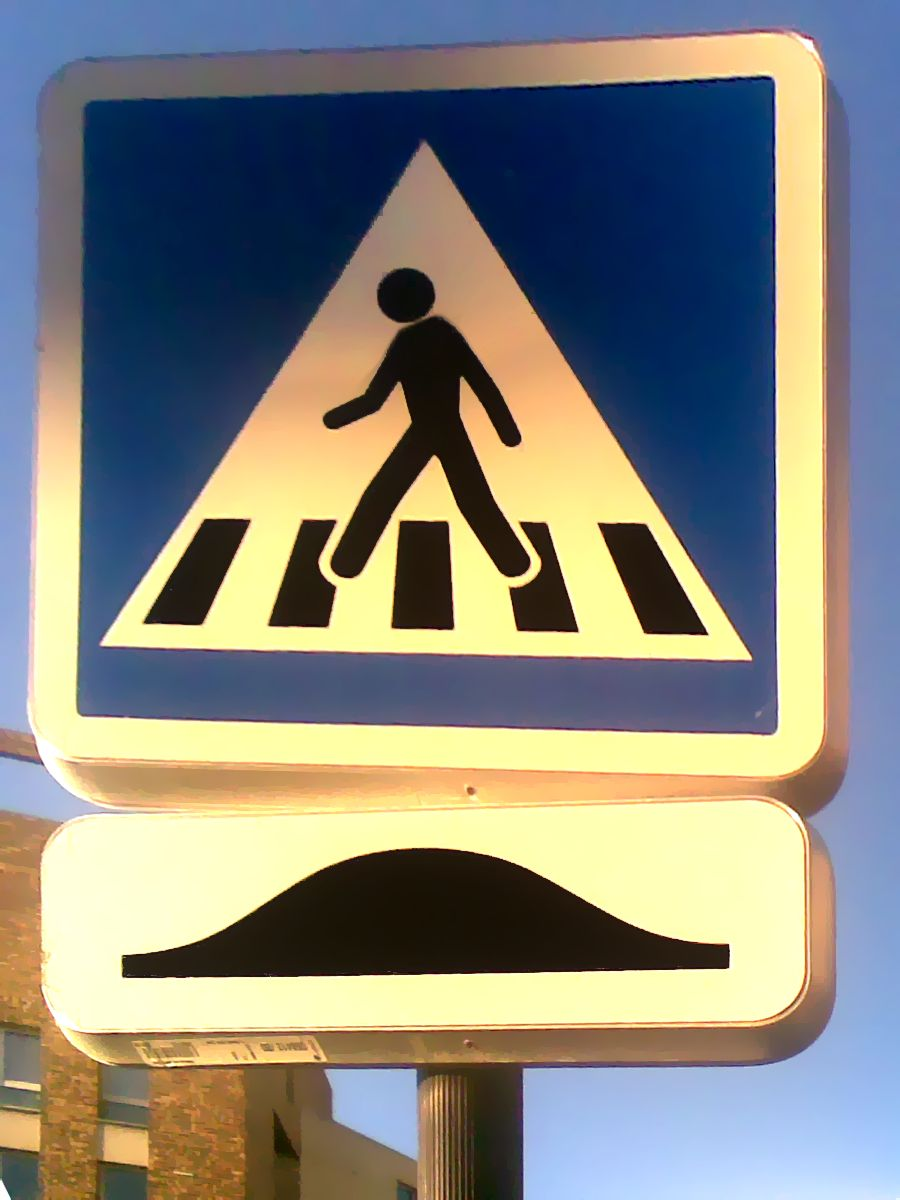
\includegraphics[width=3.3cm]{Normal-warning2.jpg}\vspace{-3ex}
\end{wrapfigure}
%Уважаемые читатели, перед вами изображён дорожный знак, который не оставит равнодушным любого человека, изучавшего математическую статистику. 
Сей дорожный знак расположен на улице Jean-Jacques Rousseau в Иври (пригород Парижа, Франция).

Объявляется конкурс на лучшее название для этого дорожного знака! Пожалуйста, присылайте свои варианты ответа в редакцию, \href{mailto:kuznesashka@gmail.com}{kuznesashka@gmail.com}. 
%Лучшие варианты будут напечатаны в следующем номере вместе с~именами авторов.

	\section{Как отцы науки коэффициенты подбирали}

%{\huge«}

<<Мои данныя состояли изъ 930~наблюденій роста совершеннолѣтнихъ дѣтей и ихъ прямыхъ восходящихъ родственниковъ, числомъ 205~составлявшихъ. Всякій разъ я превращалъ высоту женскаго стана въ эквивалентъ мужескаго и использовалъ ихъ въ преобразованномъ видѣ, дабы не вызвать упрековъ, происходящихъ отъ наличествованія разницы въ ростахъ половой природы, буде я говорилъ"=бы о среднихъ. Множитель, использованный мною, составлялъ 1,08, что равносильно прибавленію чуть менѣе чѣмъ одной двѣнадцатой части къ росту каждой женщины. Сей множитель ненамного отличается отъ оныхъ, использованныхъ иными антропологами, кои къ тому-же сами малости въ различіяхъ множителей имѣютъ; какъ-бы то ни было, онъ подходитъ къ моимъ даннымъ лучше, нежели 1,07 или 1,09. Итоговый результатъ никоимъ образомъ не относится къ тѣмъ, что зависятъ отъ этихъ минутныхъ деталей, ибо такъ сталось, что изъ-за ошибочнаго указанія расчетчикъ, которому я попервости ввѣрилъ цифры, использовалъ немного другой множитель, однако результатъ вышелъ практически одинъ въ одинъ.>>

%{\hfill \huge»}
\begin{flushright}
	\textit{Фрэнсисъ Гальтонъ}, \\
	«Регрессированіе къ посредственному при наслѣдованіи ростовъ», 1886.
\end{flushright}
	

	
\end{document}

Пэйпер: как Солнце на курс акций влияет
Hirshleifer, David, and Tyler Shumway (2003). "Good day sunshine: stock returns and the weather", Journal of Finance 58 (3), pp. 1009-1032.
Jevons Commercial crises and sun-spots
 Jevons, WS (1875). "Influence of the Sun-Spot Period on the Price of Corn".

Ящик с усами
